\documentclass{lab}

\usepackage{graphicx}
\usepackage{float}
\usepackage{soul}
\usepackage{multicol}
\usepackage{amsmath}

\addtolength{\oddsidemargin}{-.4in}
\addtolength{\evensidemargin}{-.4in}

\title{ENGG1003 - Lab Week 8}
\author{Brenton Schulz}
\date{\today}

\begin{document}
\maketitle
\begin{task}{Basic 2D Array Indexing}{}
The following 2D array:
$$x = 
\begin{bmatrix} 
4 & 5 & 6 \\
7 & 8 & 9\\
10 & 11 & 12 \\
\end{bmatrix}
$$
can be created in Python with the code:\\~\\ \texttt{x = np.array([ [4,5,6], [7,8,9], [10,11,12] ])}
\\~\\
Initialise this array in your own Python script then write additional code which uses array indexing or slicing to:
\begin{itemize}
\item Print the \texttt{4}
\item Print the \texttt{9}
\item Print the bottom row
\item Print the four values in the top left as a 2x2 array:
\begin{lstlisting}
[[4 5]
 [7 8]]
\end{lstlisting}
\end{itemize}
\end{task}

\begin{task}{Intermediate Indexing and Slicing 2D Arrays}{}
Similarly to the ``plus symbol'' example in the Week 7 Thursday lecture (slides 3-7), create a 10x10 2D array of 1s and, using array slicing, draw a 1-pixel black square along the border (edge).
\end{task}

\pagebreak

\begin{task}{More Complicated 2D Array Indexing and Slicing}{}
Draw a 1-pixel white square of side length \texttt{N}, with upper left corner at row \texttt{r} and column \texttt{c}, inside an \texttt{M}x\texttt{M} array. Note that \texttt{r=0} and \texttt{c=0} indexes the top left corner. Initialise \texttt{N}, \texttt{r}, \texttt{c}, and \texttt{M} near the start of your Python script. Confirm your method works with several different test values.
\\~\\
Implement this problem with two methods:
\begin{itemize}
	\item By writing four \texttt{for} or \texttt{while} loops which index the array elements individually - one loop for each side of the square
	\item With four applications of array slicing
\end{itemize}
~\\
For initial testing, recreate Figure \ref{fig:square} where \texttt{r=3}, \texttt{c=2}, \texttt{N=4} and \texttt{M=10}.
\\~\\
Extension: Write a function which takes \texttt{N}, \texttt{r}, \texttt{c}, and \texttt{M} as arguments and returns the array.
\begin{figure}[H]
\begin{center}
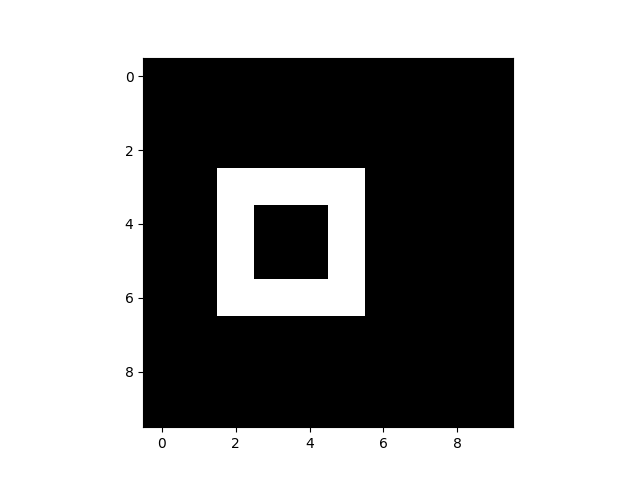
\includegraphics[width=0.8\textwidth]{square.png}
\end{center}
\caption{A square of side length 4 drawn from row index 2 and column index 3 drawn on a 10x10 2D array.}\label{fig:square}
\end{figure}
\end{task}

\pagebreak
\begin{task}{Mapping Cartesian Coordinates to 2D Array Indices}{}
Consider an autonomous robot which receives accurate position information from external sensors and needs to locate itself on a map stored in a 2D array\footnote{This is a basic form of ``occupancy mapping''.}. Assume that the external sensors provide $x$-$y$ coordinates from some known ``origin'' and that the robot is constrained to a room of known size. The origin is not necessarily in the corner of the room but can be located anywhere. The $x$ and $y$ values of the room edges are known. The robot's internal programming will require a method to calculate a 2D \texttt{row} and \texttt{column} array index given an $x$-$y$ coordinate.
\\~\\
To do this a ``mapping'' is required which converts a Cartesian point, ($x$,$y$), to an array row, \texttt{r}, and column, \texttt{c} of a matrix with \texttt{M} rows and \texttt{N} columns.
\\~\\
Consider the sketch in Figure \ref{fig:mapping}. It shows how a column index would map from a minimum value, \texttt{MIN}, at column zero, to a maximum value, \texttt{MAX}, at column \texttt{N}. When viewed from above, you can think of the \texttt{x} \texttt{MIN} and \texttt{MAX} values as the $x$ coordinate of the left and right edges of the room, respectively.
\begin{figure}[H]
\begin{center}
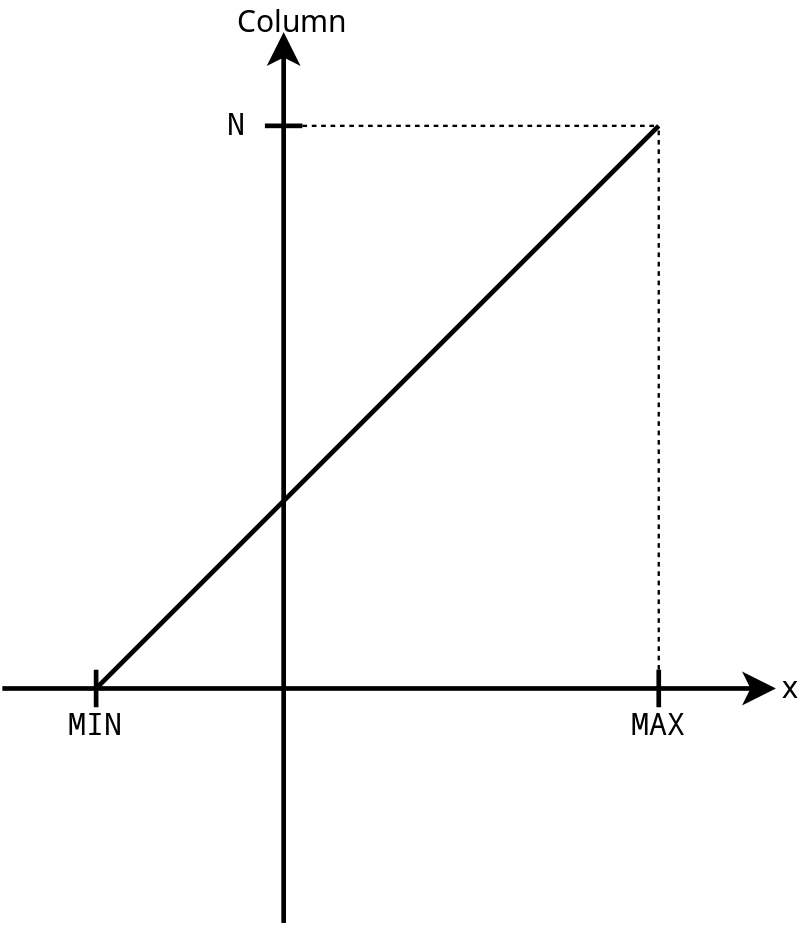
\includegraphics[width=0.46\textwidth]{mapping.png}
\end{center}
\caption{A linear mapping from an $x$ coordinate to an array column index.}\label{fig:mapping}
\end{figure}
\textbf{Task:} Applying the 2-point formula:
\begin{equation}
y = \frac{y_2 - y_1}{x_2 - x_1}(x-x_1)+y_1
\end{equation}
write an equation which converts a Cartesian $x$ coordinate to a 2D array column index. To do this, observe that the ``$x$`` in the formula is the $x$ coordinate of the robot and that ``$y$`` in the formula is the required column index. Take the point ($x_1,y_1$) to be the Figure \ref{fig:mapping} point ($\texttt{MIN}, 0$) and ($x_2,y_2$) to be the point (\texttt{MAX}, \texttt{N}), and substitute them into the 2-point formula.
\\~\\
\textbf{NB:} When implementing this formula to index an array use the built in Python function \texttt{int()} to convert the column value to an integer.
\\~\\
Repeat this method to calculate a row number given the top and bottom $y$-coordinate extremes of an image. Create your own sketch then substitude into the 2-point formula. Note that the top (ie: maximum value of $y$) now maps to row zero and the bottom (minimum value of $y$) to row \texttt{M}.
\end{task}

\begin{task}{Barnsley Fern}{}

In this task you will modify an existing Python program to generate an image of the \textit{Barnsley fern} fractal.
\\~\\
A \textit{fractal} is a mathematically generated image which exhibits ``self-similar'' geometry. As the image is zoomed in the the same patterns are seen repeated and, in theory, the image can be zoomed in forever and still show the same level of detail as it did when zoomed out.
\\~\\
The Barnsley fern is from a class of fractals known as iterated function systems (IFS). The general pattern for generating fractals of this type is to:
\begin{enumerate}
\item Pick (or be given) a point $x_0,y_0$
\item Generate a new point, $x_1,y_1$, by applying some mathematical rules
\item Draw a dot on an $x$-$y$ plane where the new point lies
\item Repeat millions (or billions) of times until an image is drawn
\end{enumerate}
~\\
The rules for the Barnsley fern are as follows:
\begin{itemize}
\item There are four functions which generate a new point, ($x_{n+1}, y_{n+1}$), from an old point ($x_n,y_x$):
	\begin{itemize}
		\item $f_1:$
		 \begin{flalign*}
x_{n+1} &= 0 &&\\
y_{n+1} &= 0.16y_n &&
		\end{flalign*}
 
		\item $f_2:$
		 \begin{flalign*}
x_{n+1} &= 0.85 x_n + 0.04y_n &&\\
y_{n+1} &= -0.04x_n + 0.85y_n + 1.6 &&
		\end{flalign*}
		\item $f_3:$
		 \begin{flalign*}
x_{n+1} &= 0.2 x_n - 0.26y_n &&\\
y_{n+1} &= 0.23x_n + 0.22 y_n + 1.6 &&
		\end{flalign*}
		\item $f_4:$
		 \begin{flalign*}
x_{n+1} &= -0.15 x_n + 0.28 y_n &&\\
y_{n+1} &= 0.26 x_n + 0.24y_n + 0.44 &&
		\end{flalign*}
	\end{itemize}
\item Each iteration, \textit{one} of the four functions is chosen at random with a probability, $p$, of:
	\begin{itemize}
		\item $f_1$: $p=0.01$
		\item $f_2$: $p=0.85$
		\item $f_3$: $p=0.07$
		\item $f_4$: $p=0.07$
	\end{itemize}
\end{itemize}
~\\
\textbf{Task:} Open the Barnsley Fern Wikipedia page: \url{https://en.wikipedia.org/wiki/Barnsley_fern}
\\~\\
Navigate to the ``Syntax examples'' section, copy the Python script (the first one) and run it (after a \texttt{pip install turtle}). Note that execution is \textit{very} slow, about 10 points per second.
\\~\\
Using your results from the previous task (or the solution at the end of this document), modify this code to draw directly to an \texttt{MxN} array instead of plotting with the \texttt{turtle} library. You will need to create your own array with \texttt{np.zeros()} then index it as-per the formulas derived earlier.
\\~\\
Use the following values for the edges of the image:
\\
\begin{itemize}
\item Left edge: $x=-2.5$
\item Right edge: $x=2.7$
\item Top edge: $y=10.0$
\item Bottom edge: $y=-0.01$
\end{itemize}
~\\
Start with a small image (say 200x200 pixels) and a small iteration count (say, 10 000) so that debugging can be performed in a reasonable time.
\\~\\
Initialise the drawing to all zeros and assign a value of 1 to every pixel the algorithm ``visits''. Plot the final image with \texttt{plt.imshow()}.
\\~\\
\textbf{Extension:} Instead of assigning 1 to each visited pixel \textit{increment} the value by 1. When plotting, use a plot command which specifies the minimum and maximum values so that the brightness and contrast are scaled correctly. eg, if the image is called \texttt{im\_gray}:\\ \texttt{plt.imshow(im\_gray,cmap='gray', vmin = 0, vmax = im\_gray.max())}
\end{task}

\section*{Coordinate to Array Index Mapping Solution}

Assuming an array with \texttt{M} rows and \texttt{N} columns:


\begin{equation}
\texttt{row} = \frac{-\texttt{M}}{\texttt{YMAX}-\texttt{YMIN}}(y-\texttt{YMIN}) + \texttt{M}
\end{equation}

\begin{equation}
\texttt{column} = \frac{\texttt{N}}{\texttt{XMAX}-\texttt{XMIN}}(x-\texttt{XMIN}) 
\end{equation}

These equations assume the following interpretations for the image edges:

\begin{itemize}
\item Top: \texttt{YMAX}
\item Bottom: \texttt{YMIN}
\item Left: \texttt{XMIN}
\item Right: \texttt{XMAX}
\end{itemize}

\textbf{NB:} Round the results with \texttt{int()}!

\end{document}
